\title{BT5110 Data Management and Warehousing}

\subtitle{Tutorial 0 Special: Foundamental \texttt{psql} Operations}

\author{Mark Meng Huasong}

\institute[National University of Singapore] % (optional, but mostly needed)
{
	School of Computing\\
	National University of Singapore
}

\titlegraphic{
	
\includegraphics[width=2cm]{nus-logo}
}

\date{Aug 2021}

\begin{frame}
	\titlepage
\end{frame}

\section*{Configuration}

\begin{frame}[fragile]{Configuration on Windows PC (8/10/11)}
	(1-a) Right click my PC, click ``Properties''. \\
	Go to ``Advanced'' tab, click the ``Environment Variables'' button.
	\begin{figure}
		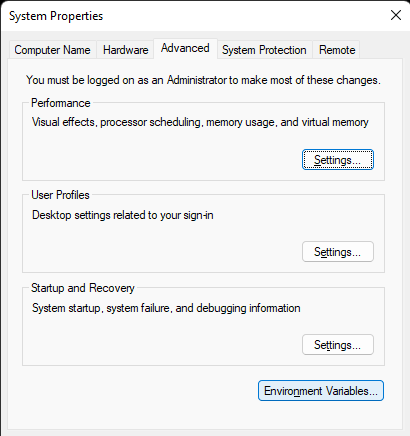
\includegraphics[width=0.5\textwidth]{t0-psql/images/settings.png}
	\end{figure}
\end{frame}

\begin{frame}[fragile]{Configuration on Windows PC}
	(1-b) Alternatively, you may also click ``start'' and type keyword to search, like the figure below:
	\begin{figure}
		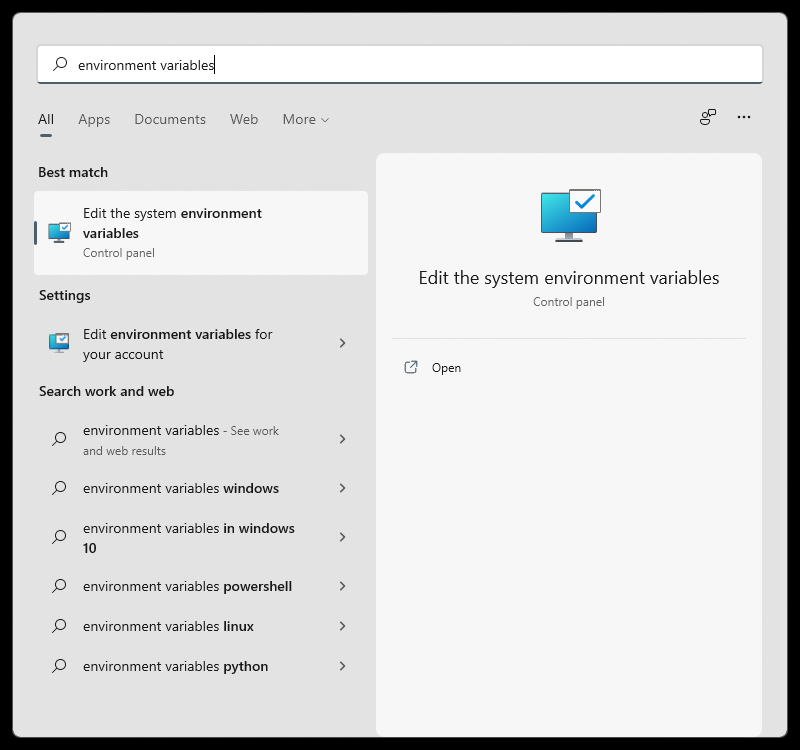
\includegraphics[width=0.5\textwidth]{t0-psql/images/start-search.png}
	\end{figure}
\end{frame}

\begin{frame}[fragile]{Configuration on Windows PC}
	(2) Find the ``Path'' in system variables.
	\begin{figure}
		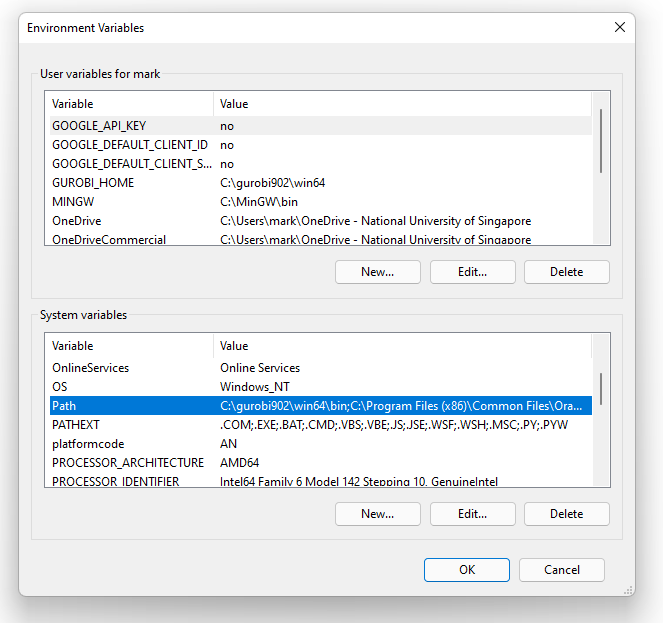
\includegraphics[width=0.5\textwidth]{t0-psql/images/environment-list.png}
	\end{figure}
\end{frame}

\begin{frame}[fragile]{Configuration on Windows PC}
	(3) Add your PostgreSQL 13 installation path \\(typically \texttt{C:\textbackslash\textbackslash Program Files\textbackslash PostgreSQL\textbackslash 13\textbackslash bin}).
	\begin{figure}
		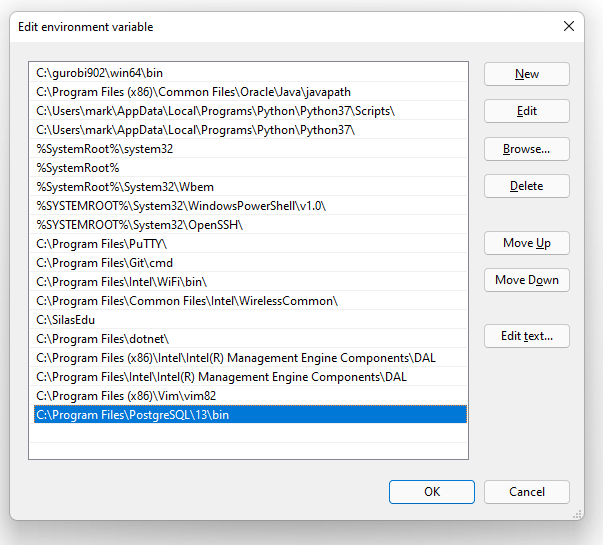
\includegraphics[width=0.5\textwidth]{t0-psql/images/path-values.png}
	\end{figure}
\end{frame}

\section*{Basic database operations}

\begin{frame}[fragile]{Connect to psql server on Windows PC}

Open ``Command Line''/``Windows Terminal'', and type in the command below to connect PostgreSQL.
\begin{figure}
	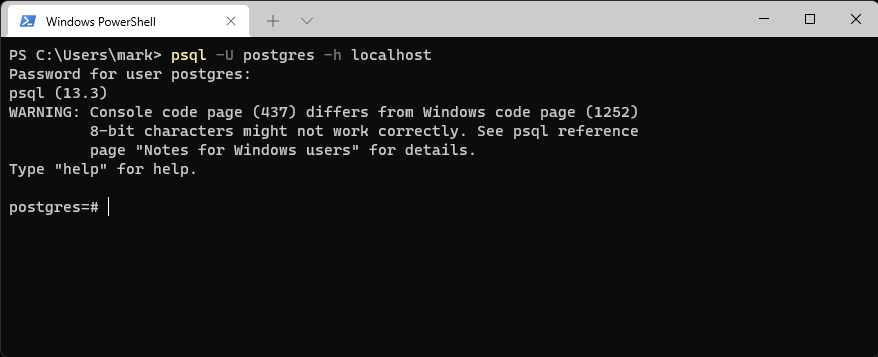
\includegraphics[width=0.7\textwidth]{t0-psql/images/1.png}
\end{figure}

\begin{alertblock}{Caution}
	Don't just enter ``\texttt{psql}'' as it assumes you are connecting with your Windows login account (e.g., \texttt{\textbf{mark}} in this case). However, in a fresh installed PostgreSQL, there is no such user but only ``\texttt{\textbf{postgres}}''. 
\end{alertblock}

\end{frame}

\begin{frame}[fragile]{Connect to psql server on Mac}
	On Mac, you can just connect to a server by double clicking the specific icon on Postgres app. \vspace{5pt}
	\begin{figure}
		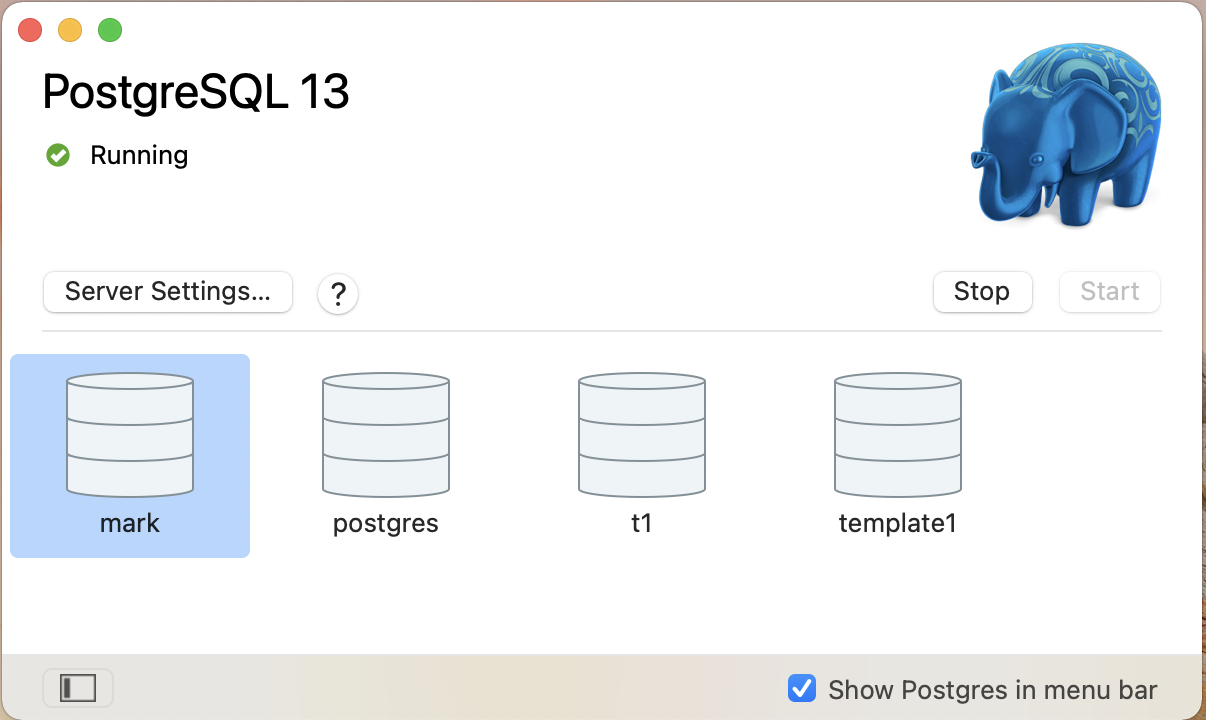
\includegraphics[width=0.4\textwidth]{t0-psql/images/mac1.png}
	\end{figure}

	If you want to launch it manually on terminal, enter command below (for Postgres 13 only):
	
	{\scriptsize \texttt{mark@mac \% /Applications/Postgres.app/Contents/Versions/13/bin/psql -p5432 ``postgres''}}
\end{frame}

\begin{frame}[fragile]{Create a new database}
	Enter ``\texttt{create database abc;}'' to \textbf{create} a database named ``abc''.
	\begin{figure}
		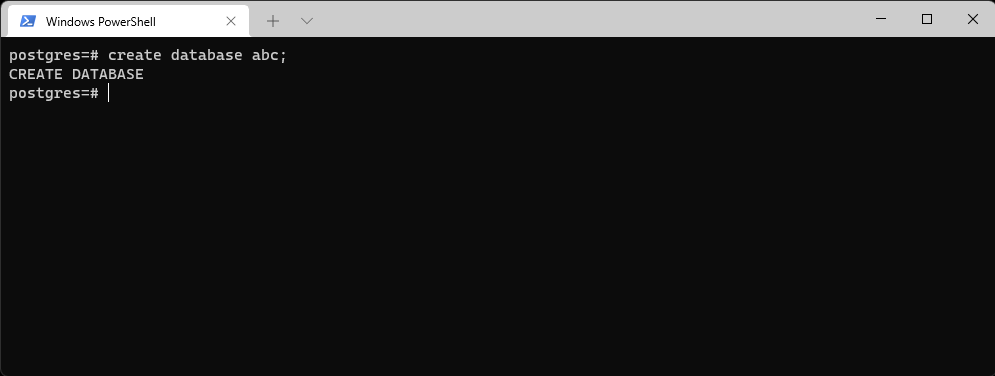
\includegraphics[width=0.85\textwidth]{t0-psql/images/3.png}
	\end{figure}
	
\end{frame}

\begin{frame}[fragile]{Browse all databases}
	Enter ``\texttt{\textbackslash l}'' to \textbf{list} all databases.
	\begin{figure}
		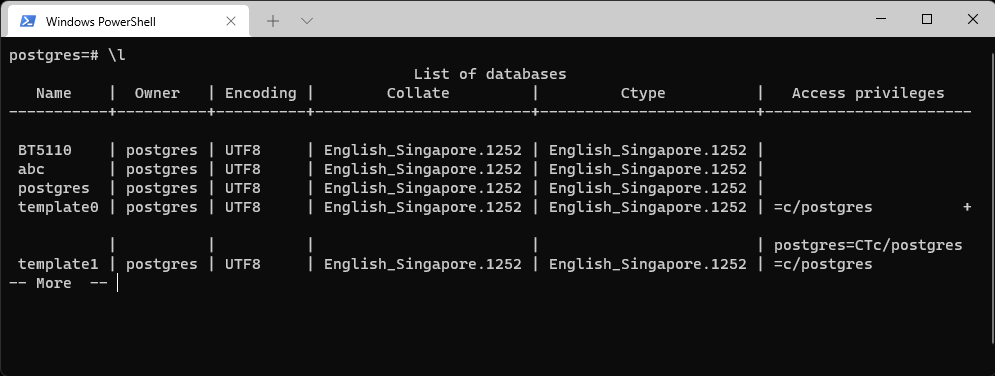
\includegraphics[width=0.85\textwidth]{t0-psql/images/2.png}
	\end{figure}
	
\end{frame}

\begin{frame}[fragile]{Connect to a database}
	Enter ``\texttt{\textbackslash c abc}'' to \textbf{connect} with the database ``abc''.
	\begin{figure}
		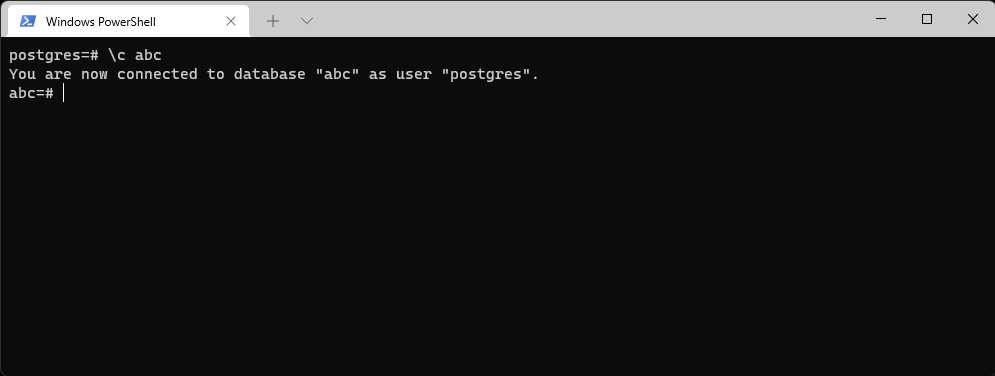
\includegraphics[width=0.85\textwidth]{t0-psql/images/4.png}
	\end{figure}
	
\end{frame}

\begin{frame}[fragile]{Create a table}
	Let's create a table ``student'', which is exactly same as the one we will use for Tutorial 1.
	\begin{figure}
		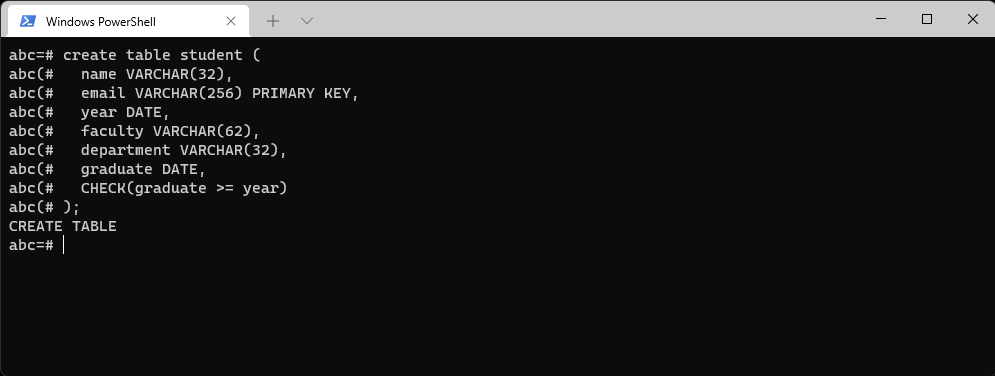
\includegraphics[width=0.8\textwidth]{t0-psql/images/5.png}
	\end{figure}
	
\end{frame}

\begin{frame}[fragile]{View existing tables}
	
	Enter ``\texttt{\textbackslash d}'' to \textbf{display} all relations in the current database.\\
	Enter ``\texttt{\textbackslash d student}'' to \textbf{display} the details of the table ``\texttt{student}''.
	\begin{figure}
		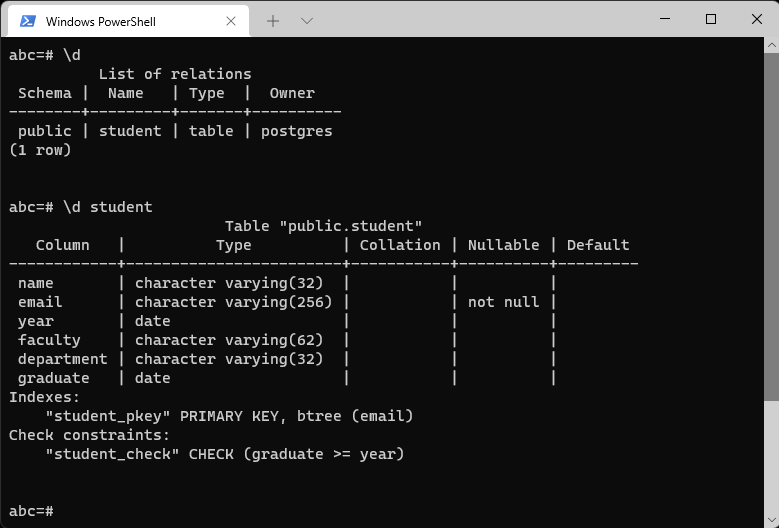
\includegraphics[width=0.8\textwidth]{t0-psql/images/6.png}
	\end{figure}
		
\end{frame}

\begin{frame}[fragile]{Execute an SQL script from files}
	Now let's insert some data. To save time, we just make use of the SQL script provided for our tutorials -- ``\texttt{NUNStAStudent.sql}''
	
	\begin{figure}
		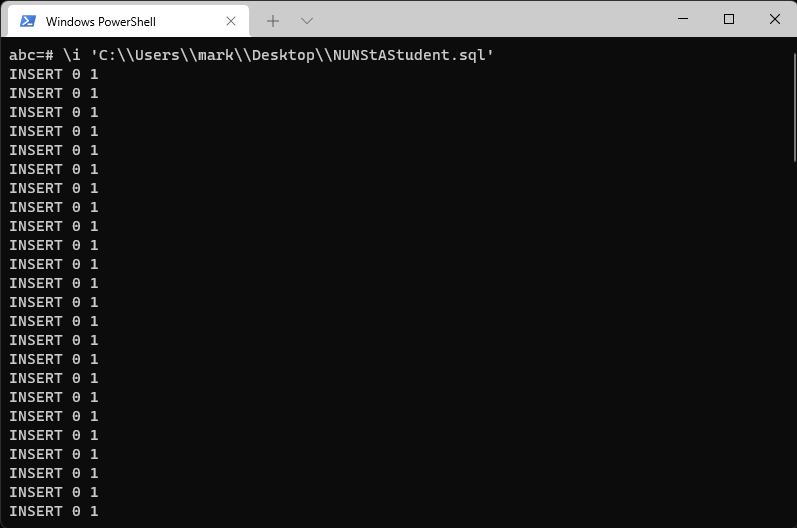
\includegraphics[trim=0 5cm 0 0, clip, width=0.65\textwidth]{t0-psql/images/7.png}
	\end{figure}
	
	\begin{alertblock}{Caution (Windows only)}
		Please be cautious that the file path on Windows must be formatted with double `//' and enclosed within single-quote symbols (``\textit{C:\textbackslash\textbackslash Users\textbackslash\textbackslash mark\textbackslash\textbackslash Desktop\textbackslash\textbackslash NUNStAStudent.sql }'' in this case). Otherwise a \texttt{Permission Denied} error will be returned.
	\end{alertblock}
	
\end{frame}

\begin{frame}[fragile]{Execute an SQL script from files (Cont.)}
	On Mac, you can just drag the file to the terminal, the path is automatically formatted.\vspace{20pt}
	
	E.g., \texttt{abc=\# \textbackslash i /Users/mark/Documents/NUNStAStudent.sql}
	
\end{frame}


\begin{frame}[fragile]{Execute an SQL script manually}
	
	Enter SQL query manually to view outputs.
	\begin{figure}
		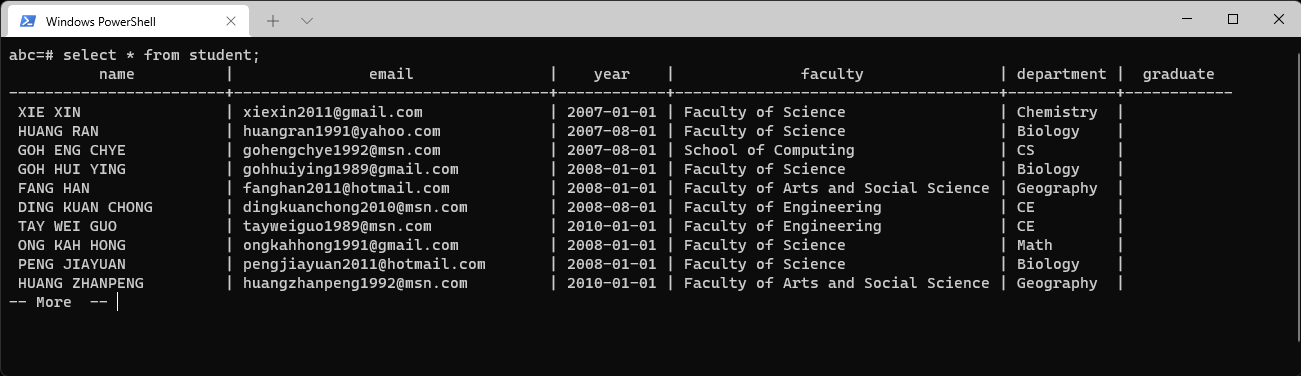
\includegraphics[width=0.9\textwidth]{t0-psql/images/8.png}\vspace{10pt}
		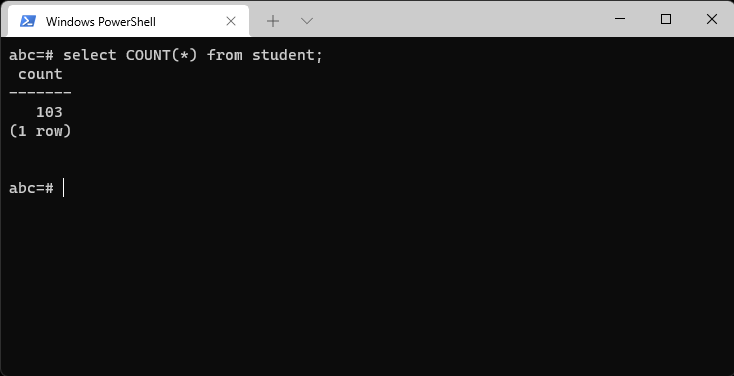
\includegraphics[width=0.5\textwidth]{t0-psql/images/9.png}
	\end{figure}
	
\end{frame}

\begin{frame}[fragile]{Disconnect \& Drop a database}
	
	To drop the current database, you have to disconnect it first.\\
	To do that, just connect to the other one by entering ``\texttt{\textbackslash c postgres}'' to \textbf{connect} to the default database ``\texttt{postgres}''.\\
	Then enter ``\texttt{drop database abc}'' to \textbf{drop} the database we have just created.
	
	\begin{figure}
		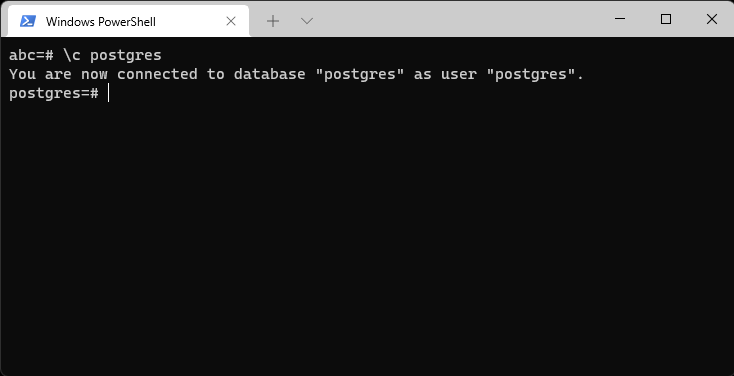
\includegraphics[trim=0 5cm 0 0, clip, width=0.7\textwidth]{t0-psql/images/10.png}\vspace{10pt}
		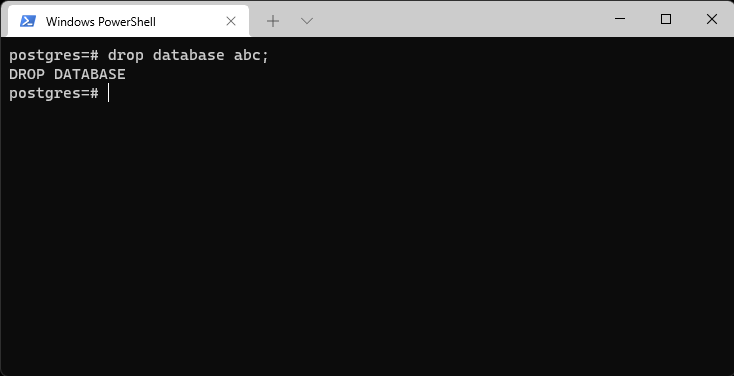
\includegraphics[trim=0 5cm 0 0, clip, width=0.7\textwidth]{t0-psql/images/11.png}
	\end{figure}
	
\end{frame}

\begin{frame}[fragile]{Quit the \texttt{psql}}
	
	Enter ``\texttt{\textbackslash q}'' to \textbf{quit}.
	\begin{figure}
		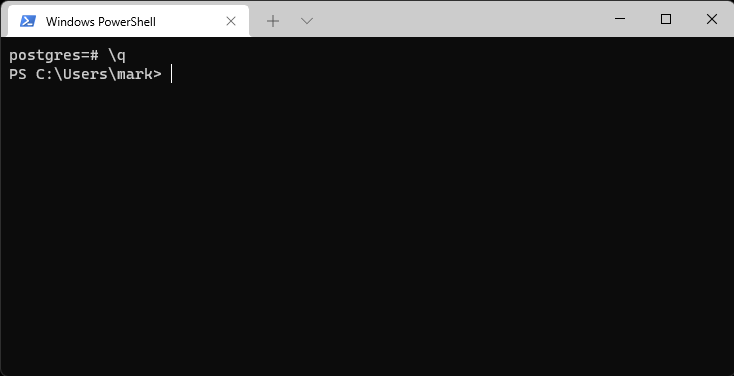
\includegraphics[width=0.85\textwidth]{t0-psql/images/12.png}
	\end{figure}
	
\end{frame}
\begin{frame}{}
\centering  
For any further question, please feel free to email me:\vspace{10pt}

hmeng@comp.nus.edu.sg \vspace{20pt}

\end{frame}